\subsection*{Digital Divider}


\begin{figure}[H]
\centering
\tikzstyle{dot} = [draw,shape=circle,fill=black, scale =.3]
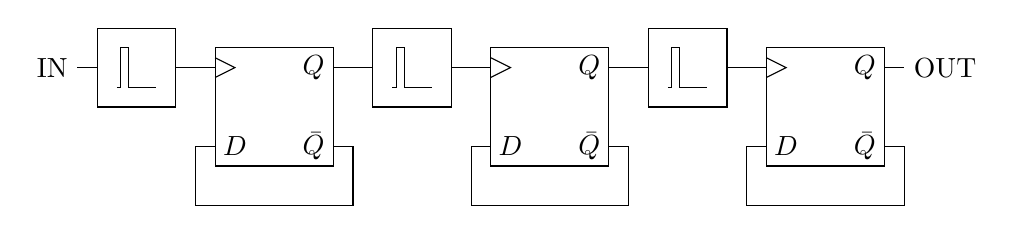
\begin{tikzpicture}
%%% entire block
% DFF Block
\draw  (-1.5,1) rectangle (0,-0.5);
\draw (-1.5,0.875) to (-1.25,0.75) to (-1.5,0.625);
\node at (-1.25,-0.25) {$D$};
\node at (-0.25,0.75) {$Q$};
\node at (-0.25,-0.25) {$\bar{Q}$};

% connections
\draw (0,-0.25) -| (0.25,-1) -- (-1.75,-1) |- (-1.5,-0.25);
\draw (-1.5,0.75) -- (-2,0.75);
\draw (-3,0.75) -- (-3.25,0.75);

% pulse generator
\draw (-2.75,0.5) -| (-2.7,1) -| (-2.6,0.5) -- (-2.25,0.5);
\draw  (-3,1.25) rectangle (-2,0.25);

%%% entire block
% DFF Block
\draw  (2,1) rectangle (3.5,-0.5);
\draw (2,0.875) to (2.25,0.75) to (2,0.625);
\node at (2.25,-0.25) {$D$};
\node at (3.25,0.75) {$Q$};
\node at (3.25,-0.25) {$\bar{Q}$};

% connections
\draw (3.5,-0.25) -| (3.75,-1) -- (1.75,-1) |- (2,-0.25);
\draw (2,0.75) -- (1.5,0.75);
\draw (0.5,0.75) -- (0,0.75);

% pulse generator
\draw (0.75,0.5) -| (0.8,1) -| (0.9,0.5) -- (1.25,0.5);
\draw  (0.5,1.25) rectangle (1.5,0.25);

%%% entire block
% DFF Block
\draw  (5.5,1) rectangle (7,-0.5);
\draw (5.5,0.875) to (5.75,0.75) to (5.5,0.625);
\node at (5.75,-0.25) {$D$};
\node at (6.75,0.75) {$Q$};
\node at (6.75,-0.25) {$\bar{Q}$};

% connections
\draw (7,-0.25) -| (7.25,-1) -- (5.25,-1) |- (5.5,-0.25);
\draw (5.5,0.75) -- (5,0.75);
\draw (4,0.75) -- (3.5,0.75);

% pulse generator
\draw (4.25,0.5) -| (4.3,1) -| (4.4,0.5) -- (4.75,0.5);
\draw  (4,1.25) rectangle (5,0.25);


%in and out
\draw(7,0.75) -- (7.25,0.75);
\node [anchor=east] at (-3.25,0.75) {IN};
\node [anchor=west]  at (7.25,0.75) {OUT};
\end{tikzpicture}

\caption{Digital divider}
\label{tkz:digitalDivider}
\end{figure}